\section{The physical theory behind Secondary Frequency Control} %3.1

From Chapter~\ref{Chapter2}, we mentioned that disturbances occur in the system, there be a distortion in the power balance between that delivered by the turbines and that consumed by the loads. The imbalance is from the kinetic energy of rotating rotors of turbines, generators and motors and, thus, the frequency in the system change. If no control is applied, the frequency largely deviates and then reaches a meagre and steady-state value, due to which the electrical grid is shut down.  

We also mentioned that the system will start Primary Frequency Control firstly and then the frequency will remain at a steady-state value below or above the nominal one. After that, Secondary Frequency Control starts. 

The mechanism of Secondary Frequency Control is to restore the frequency to the nominal one. 

Secondary frequency control, or load frequency control (LFC), or automatic generation control (AGC), is an automatic control that restores the frequency back to its nominal value in a centralised way. It's implemented that is activated after the primary frequency control. Typically, it takes 30 seconds to 15 minutes. 

\begin{figure*}[htbp]
\centering
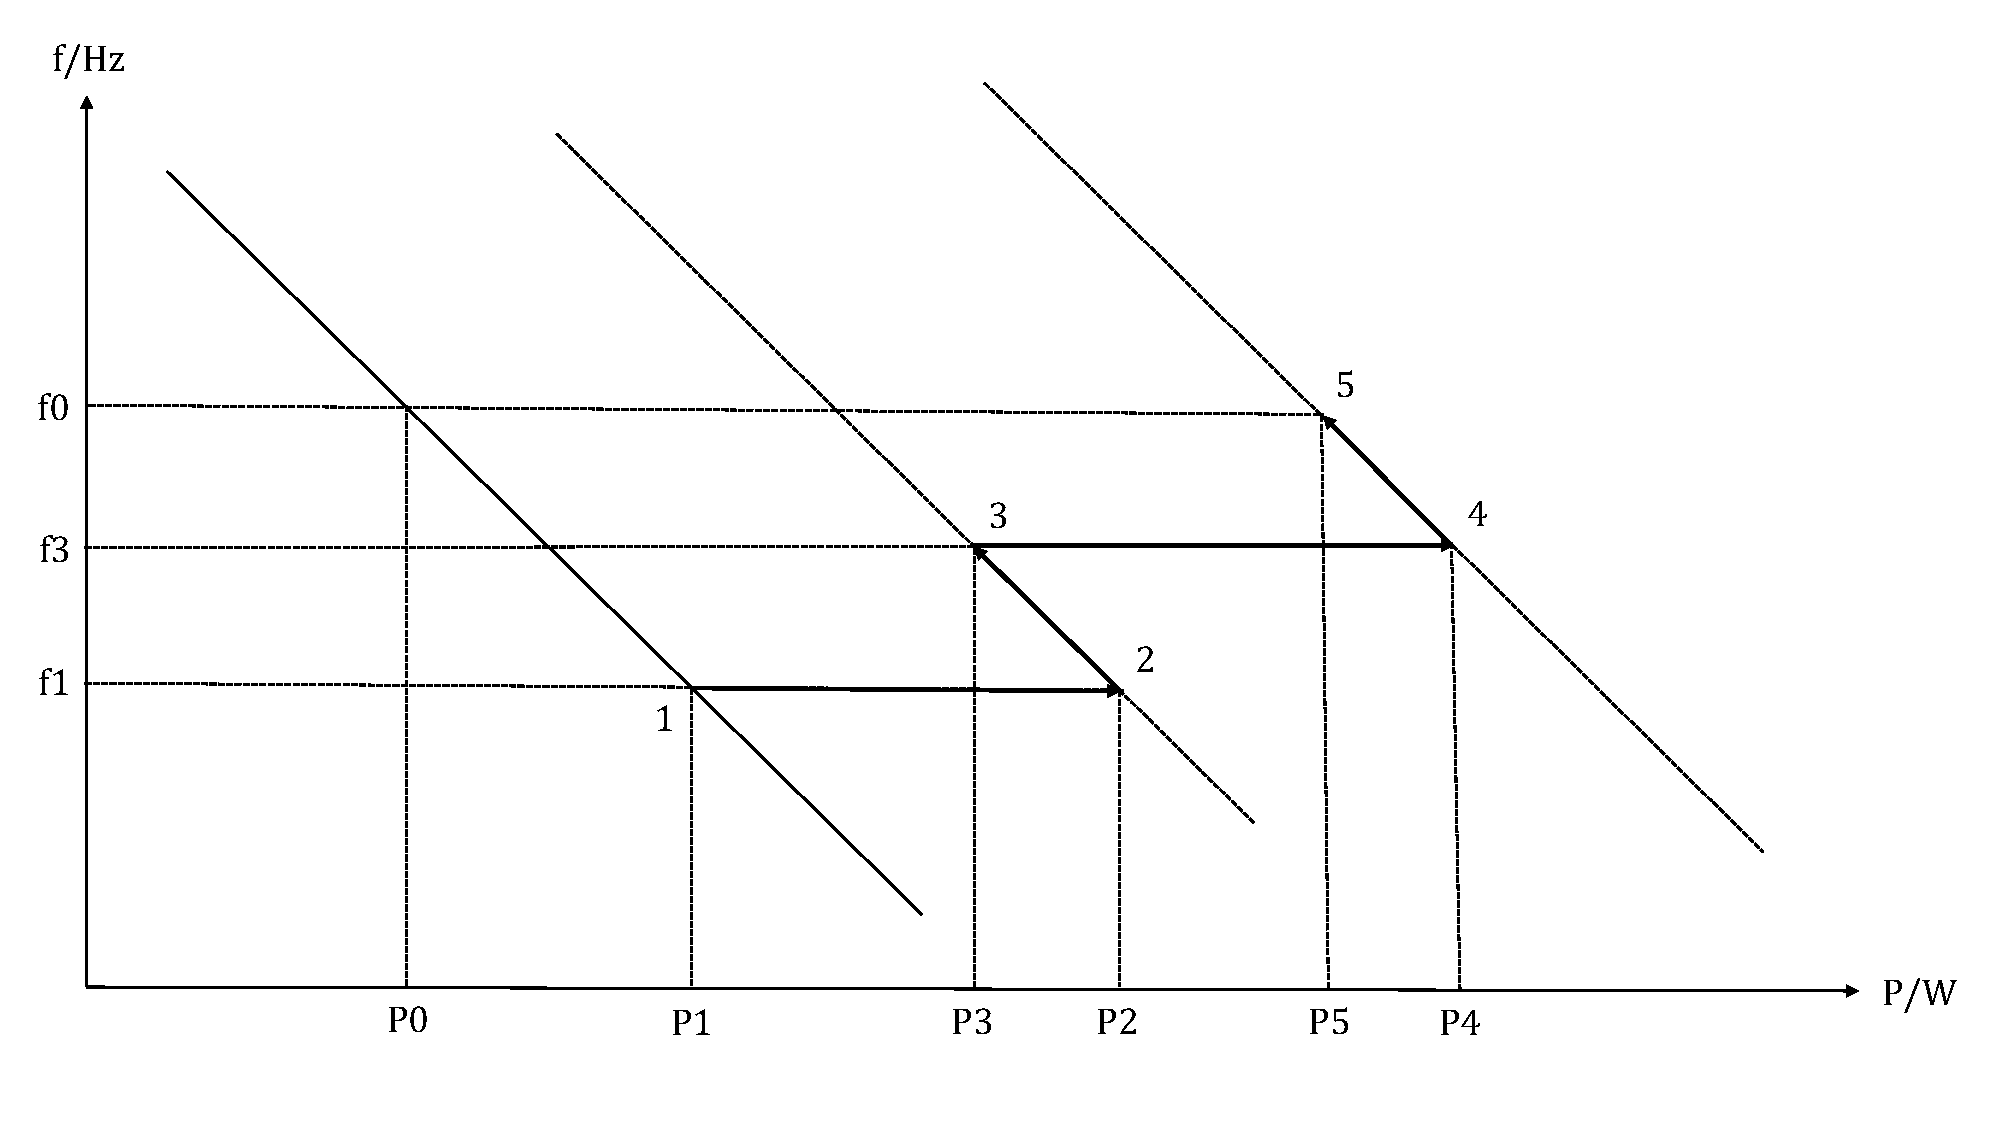
\includegraphics[width = 0.816\textwidth]{figure/3_1_Equilibrium.pdf}
\caption{Equilibrium points for an increase in the power demand.}
\label{3_1_Equilibrium}
\end{figure*}

According to Figure~\ref{3_1_Equilibrium}, frequency value rise when reference power rises. Assumed point 1 is the situation after primary frequency control happens and point 5 has the nominal value of frequency. When trying to raise the reference power a little bit, point 1 shift to point 2. Due to the power rise, the frequency of the system rise, so point 2 move to point 3. Changing more reference power of individual governors move the overall generation characteristic of the system upwards. Eventually, this lead to the restoration of the rated frequency ($f0$). 

\begin{figure}[htb]
\centering
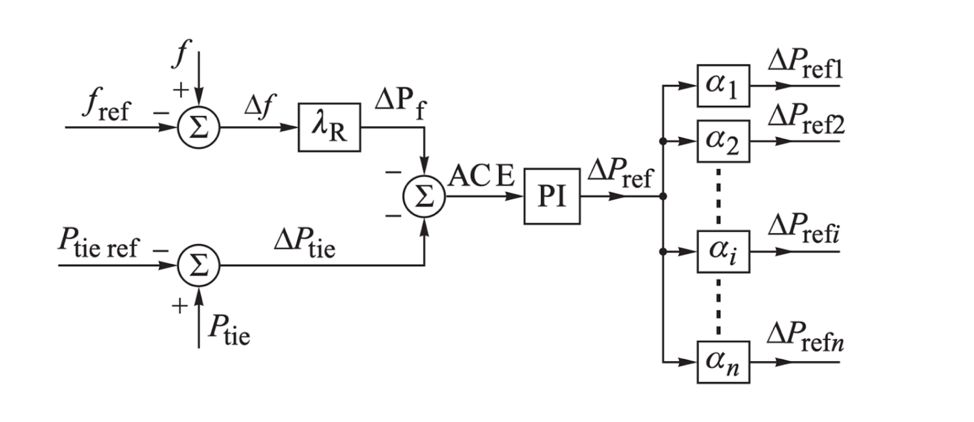
\includegraphics[width = 0.891\textwidth]{figure/3_1_Functional.png}
\caption{Functional diagram of a central regulator.}
\label{3_1_Functional}
\end{figure}

As seen in Figure~\ref{3_1_Functional}, the frequency ($f$) be measured in the local network and compared with the reference frequency to produce an amplified signal ($\Delta P_f$) that is proportional to the frequency deviation ($\Delta f$). For instance, if the frequency is smaller the reference frequency, then the signal $\Delta P_f$ be negative. Thus, input signal ACE is positive according to the functional diagram. Therefore, output signal $\Delta P_f$ is positive and it adjust the system by raising the reference value of the power. Then the system have a new frequency value ($f_{n e w}$) that go through the functional diagram again to compare the difference with the value of the reference frequency. ACE won’t be zero and the frequency won’t be stopped adding until we remove any error. 

In this standard case, which ignores the existence of tie-line interchange error, the only condition to remove errors is the frequency deviation ($\Delta f$) equals to zero. 

\begin{figure}[htbp]
\centering
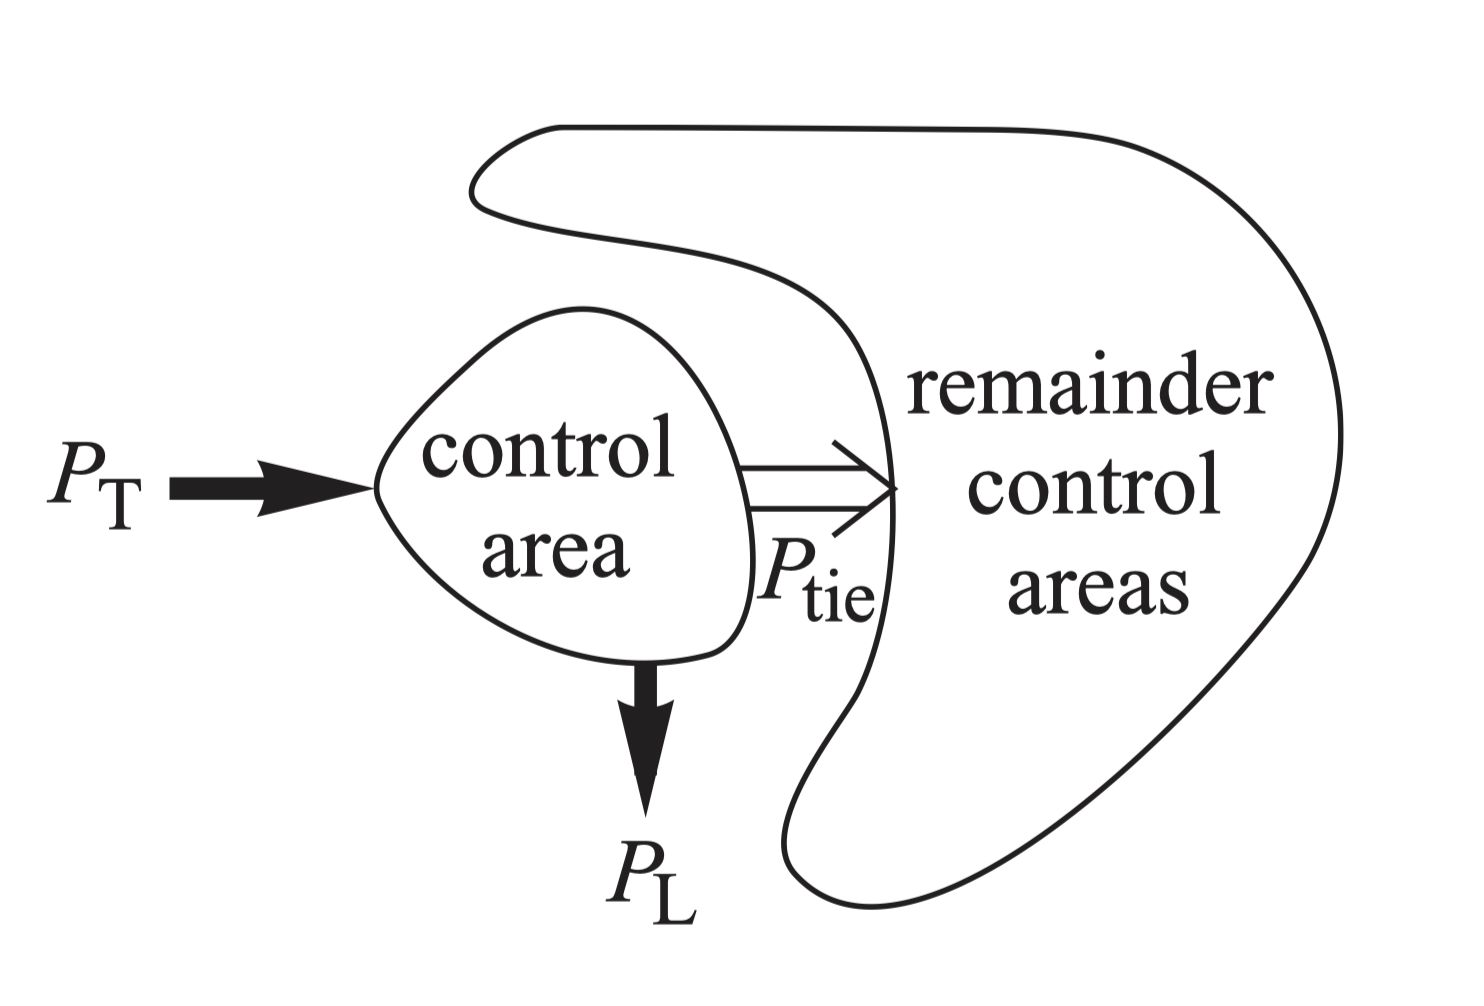
\includegraphics[width =0.819\textwidth]{figure/3_1_Power.png}
\caption{Power balance of a control area.}
\label{3_1_Power}
\end{figure}

However, it would be more difficult if consider the situation of tie-line interchange error. In interconnected power systems, AGC is implemented in a way where each subsystem has its own regulator. As shown in Figure~\ref{3_1_Power}, the power system is in equilibrium if the total power generation ($P_T$), the total power demand ($P_L$) and the net tie-line interchange power ($P_{t i e}$) satisfy the condition in each subsystem: 

\begin{equation} \label{eq1}
P_T - (P_L + P_{t i e}) = 0
\end{equation}

The objective of each regulator of the subsystem is to maintain frequency at the nominal level and to maintain net tie-line interchanges from the given area at the scheduled values. If there is a disturbance in one subsystem, then regulators in each subsystem should try to restore the frequency and net tie-line interchanges. Each subsystem regulator should enforce an increased generation covering its own area power imbalance and maintain planned net tie-line interchanges.

As shown in Figure~\ref{3_1_Functional}, to obtain a signal proportional to the tie-line interchange error $(\Delta P_{tie})$, the information on power flows in the tie-lines is sent via telecommunication lines to the central regulator which compares it with the reference value. Then the signal $(\Delta P_f)$ is added to the net tie-line interchange error $(\Delta P_{tie})$ so that ACE is


\begin{equation} \label{eq2}
ACE = - \Delta P_f - \Delta P_{tie}
\end{equation}


The situation here is similar to the situation above, where we ignore tie-line interchange error, except for the condition to remove errors. In this book, it shows us zeroing of errors can be achieved in two ways: zeroing of both errors ($ P_{tie} = 0 $ and $ f = 0 $) and achieving a compromise between the errors ($\Delta P_f + P_{tie} = 0$ or $P_f = - \Delta P_{tie}$). 